\documentclass[aspectratio=169]{beamer}

% \includeonlyframes{current}

\usepackage[T1]{fontenc}
\usepackage[utf8]{inputenc}
\usepackage{unicode}
\usepackage[american]{babel}
\usepackage{amsmath,amsthm}
\usepackage{array}
\usepackage{ifthen}
\usepackage{tikz}
\usetikzlibrary{matrix,decorations,decorations.text,calc,arrows,snakes,shapes,positioning}

\usepackage[nosfdefault]{comicneue}
\usepackage{sourcesanspro}
\usepackage[amssymb,amsfonts]{concmath}
\usefonttheme[onlymath]{serif}
\usepackage{ulem}

\mode<presentation>{%
  \usetheme{Boadilla}
}
\beamertemplatenavigationsymbolsempty
\usecolortheme[RGB={0,98,255}]{structure}
\definecolor{title}{RGB}{0,98,255}
\setbeamercolor*{title}{fg=title}

\renewcommand{\emph}[1]{{\usebeamercolor[fg]{structure}#1}}

\newcommand{\C}{ℂ}
\newcommand{\R}{ℝ}
\newcommand{\Z}{ℤ}
\newcommand{\N}{ℕ}
\newcommand{\Q}{ℚ}
\newcommand{\F}{\mathbb{F}}
\renewcommand{\P}{\mathbb{P}}
\renewcommand{\O}{\mathcal{O}}
\newcommand{\tildO}{\mathcal{\tilde{O}}}
\newcommand{\poly}{\operatorname{poly}}
\newcommand{\polylog}{\operatorname{polylog}}
\newcommand{\End}{\operatorname{End}}
\newcommand{\Hom}{\operatorname{Hom}}
\newcommand{\Gal}{\operatorname{Gal}}
\newcommand{\chr}{\operatorname{char}}
\newcommand{\Cl}{\operatorname{Cl}}
\newcommand{\GL}{\operatorname{GL}}
\renewcommand{\a}{{\mathfrak{a}}}
\renewcommand{\b}{{\mathfrak{b}}}
\newcommand{\cyc}[1]{{〈 #1 〉}}
\newcommand{\ord}{\operatorname{ord}}
\newcommand{\mat}[1]{\left(\begin{smallmatrix}#1\end{smallmatrix}\right)}

\newcommand{\bl}[1]{\textcolor{blue}{#1}}
\newcommand{\rd}[1]{\textcolor{red}{#1}}
\newcommand{\gr}[1]{\textcolor{green}{#1}}
\newcommand{\og}[1]{\textcolor{orange}{#1}}

\newcommand{\myedge}[3]{
  \draw[#3] (360/\crater*#1 : \diam) to[bend right] (360/\crater*#2 : \diam);
}
\newcommand{\sk}[4]{
  \draw[very thick,blue]   (0,0) -- (0,#1);
  \draw[very thick,red]    (1,0) -- (1,#2);
  \draw[very thick,green]  (2,0) -- (2,#3);
  \draw[very thick,orange] (3,0) -- (3,#4);
}

\newcommand\isoggraph{
    \node[circle,inner sep=.7pt,fill=black] (curve0000) at (4.1000,0.0000) {};
    \node[circle,inner sep=.7pt,fill=black] (curve0158) at (3.9895,0.9455) {};
    \node[circle,inner sep=.7pt,fill=black] (curve0410) at (3.6639,1.8401) {};
    \node[circle,inner sep=.7pt,fill=black] (curve0368) at (3.1408,2.6354) {};
    \node[circle,inner sep=.7pt,fill=black] (curve0404) at (2.4484,3.2887) {};
    \node[circle,inner sep=.7pt,fill=black] (curve0075) at (1.6239,3.7647) {};
    \node[circle,inner sep=.7pt,fill=black] (curve0144) at (0.7120,4.0377) {};
    \node[circle,inner sep=.7pt,fill=black] (curve0191) at (-0.2384,4.0931) {};
    \node[circle,inner sep=.7pt,fill=black] (curve0174) at (-1.1759,3.9278) {};
    \node[circle,inner sep=.7pt,fill=black] (curve0413) at (-2.0500,3.5507) {};
    \node[circle,inner sep=.7pt,fill=black] (curve0379) at (-2.8136,2.9822) {};
    \node[circle,inner sep=.7pt,fill=black] (curve0124) at (-3.4255,2.2530) {};
    \node[circle,inner sep=.7pt,fill=black] (curve0199) at (-3.8527,1.4023) {};
    \node[circle,inner sep=.7pt,fill=black] (curve0390) at (-4.0723,0.4760) {};
    \node[circle,inner sep=.7pt,fill=black] (curve0029) at (-4.0723,-0.4760) {};
    \node[circle,inner sep=.7pt,fill=black] (curve0220) at (-3.8527,-1.4023) {};
    \node[circle,inner sep=.7pt,fill=black] (curve0295) at (-3.4255,-2.2530) {};
    \node[circle,inner sep=.7pt,fill=black] (curve0040) at (-2.8136,-2.9822) {};
    \node[circle,inner sep=.7pt,fill=black] (curve0006) at (-2.0500,-3.5507) {};
    \node[circle,inner sep=.7pt,fill=black] (curve0245) at (-1.1759,-3.9278) {};
    \node[circle,inner sep=.7pt,fill=black] (curve0228) at (-0.2384,-4.0931) {};
    \node[circle,inner sep=.7pt,fill=black] (curve0275) at (0.7120,-4.0377) {};
    \node[circle,inner sep=.7pt,fill=black] (curve0344) at (1.6239,-3.7647) {};
    \node[circle,inner sep=.7pt,fill=black] (curve0015) at (2.4484,-3.2887) {};
    \node[circle,inner sep=.7pt,fill=black] (curve0051) at (3.1408,-2.6354) {};
    \node[circle,inner sep=.7pt,fill=black] (curve0009) at (3.6639,-1.8401) {};
    \node[circle,inner sep=.7pt,fill=black] (curve0261) at (3.9895,-0.9455) {};
    %
    \draw[color=blue] (curve0199) edge[bend right=4mm] (curve0390);
    \draw[color=blue] (curve0051) edge[bend right=4mm] (curve0009);
    \draw[color=blue] (curve0368) edge[bend right=4mm] (curve0404);
    \draw[color=blue] (curve0245) edge[bend right=4mm] (curve0228);
    \draw[color=blue] (curve0029) edge[bend right=4mm] (curve0220);
    \draw[color=blue] (curve0174) edge[bend right=4mm] (curve0413);
    \draw[color=blue] (curve0261) edge[bend right=4mm] (curve0000);
    \draw[color=blue] (curve0379) edge[bend right=4mm] (curve0124);
    \draw[color=blue] (curve0006) edge[bend right=4mm] (curve0245);
    \draw[color=blue] (curve0158) edge[bend right=4mm] (curve0410);
    \draw[color=blue] (curve0228) edge[bend right=4mm] (curve0275);
    \draw[color=blue] (curve0275) edge[bend right=4mm] (curve0344);
    \draw[color=blue] (curve0015) edge[bend right=4mm] (curve0051);
    \draw[color=blue] (curve0191) edge[bend right=4mm] (curve0174);
    \draw[color=blue] (curve0144) edge[bend right=4mm] (curve0191);
    \draw[color=blue] (curve0404) edge[bend right=4mm] (curve0075);
    \draw[color=blue] (curve0009) edge[bend right=4mm] (curve0261);
    \draw[color=blue] (curve0295) edge[bend right=4mm] (curve0040);
    \draw[color=blue] (curve0410) edge[bend right=4mm] (curve0368);
    \draw[color=blue] (curve0413) edge[bend right=4mm] (curve0379);
    \draw[color=blue] (curve0040) edge[bend right=4mm] (curve0006);
    \draw[color=blue] (curve0075) edge[bend right=4mm] (curve0144);
    \draw[color=blue] (curve0220) edge[bend right=4mm] (curve0295);
    \draw[color=blue] (curve0390) edge[bend right=4mm] (curve0029);
    \draw[color=blue] (curve0344) edge[bend right=4mm] (curve0015);
    \draw[color=blue] (curve0124) edge[bend right=4mm] (curve0199);
    \draw[color=blue] (curve0000) edge[bend right=4mm] (curve0158);
    %
    \draw[color=red] (curve0009) edge[bend right=8mm] (curve0379);
    \draw[color=red] (curve0124) edge[bend right=8mm] (curve0015);
    \draw[color=red] (curve0006) edge[bend right=8mm] (curve0368);
    \draw[color=red] (curve0228) edge[bend right=8mm] (curve0075);
    \draw[color=red] (curve0245) edge[bend right=8mm] (curve0404);
    \draw[color=red] (curve0029) edge[bend right=8mm] (curve0261);
    \draw[color=red] (curve0220) edge[bend right=8mm] (curve0000);
    \draw[color=red] (curve0368) edge[bend right=8mm] (curve0220);
    \draw[color=red] (curve0144) edge[bend right=8mm] (curve0006);
    \draw[color=red] (curve0261) edge[bend right=8mm] (curve0124);
    \draw[color=red] (curve0191) edge[bend right=8mm] (curve0245);
    \draw[color=red] (curve0015) edge[bend right=8mm] (curve0174);
    \draw[color=red] (curve0344) edge[bend right=8mm] (curve0191);
    \draw[color=red] (curve0275) edge[bend right=8mm] (curve0144);
    \draw[color=red] (curve0158) edge[bend right=8mm] (curve0390);
    \draw[color=red] (curve0295) edge[bend right=8mm] (curve0158);
    \draw[color=red] (curve0075) edge[bend right=8mm] (curve0040);
    \draw[color=red] (curve0174) edge[bend right=8mm] (curve0228);
    \draw[color=red] (curve0000) edge[bend right=8mm] (curve0199);
    \draw[color=red] (curve0379) edge[bend right=8mm] (curve0344);
    \draw[color=red] (curve0390) edge[bend right=8mm] (curve0009);
    \draw[color=red] (curve0040) edge[bend right=8mm] (curve0410);
    \draw[color=red] (curve0410) edge[bend right=8mm] (curve0029);
    \draw[color=red] (curve0404) edge[bend right=8mm] (curve0295);
    \draw[color=red] (curve0413) edge[bend right=8mm] (curve0275);
    \draw[color=red] (curve0051) edge[bend right=8mm] (curve0413);
    \draw[color=red] (curve0199) edge[bend right=8mm] (curve0051);
    %
    \draw[color=green] (curve0158) edge[bend left=10mm] (curve0144);
    \draw[color=green] (curve0009) edge[bend left=10mm] (curve0368);
    \draw[color=green] (curve0124) edge[bend left=10mm] (curve0295);
    \draw[color=green] (curve0174) edge[bend left=10mm] (curve0390);
    \draw[color=green] (curve0368) edge[bend left=10mm] (curve0174);
    \draw[color=green] (curve0344) edge[bend left=10mm] (curve0000);
    \draw[color=green] (curve0144) edge[bend left=10mm] (curve0124);
    \draw[color=green] (curve0295) edge[bend left=10mm] (curve0275);
    \draw[color=green] (curve0029) edge[bend left=10mm] (curve0245);
    \draw[color=green] (curve0051) edge[bend left=10mm] (curve0410);
    \draw[color=green] (curve0015) edge[bend left=10mm] (curve0158);
    \draw[color=green] (curve0275) edge[bend left=10mm] (curve0261);
    \draw[color=green] (curve0075) edge[bend left=10mm] (curve0379);
    \draw[color=green] (curve0379) edge[bend left=10mm] (curve0220);
    \draw[color=green] (curve0220) edge[bend left=10mm] (curve0228);
    \draw[color=green] (curve0006) edge[bend left=10mm] (curve0015);
    \draw[color=green] (curve0191) edge[bend left=10mm] (curve0199);
    \draw[color=green] (curve0228) edge[bend left=10mm] (curve0009);
    \draw[color=green] (curve0040) edge[bend left=10mm] (curve0344);
    \draw[color=green] (curve0261) edge[bend left=10mm] (curve0404);
    \draw[color=green] (curve0404) edge[bend left=10mm] (curve0413);
    \draw[color=green] (curve0390) edge[bend left=10mm] (curve0006);
    \draw[color=green] (curve0000) edge[bend left=10mm] (curve0075);
    \draw[color=green] (curve0245) edge[bend left=10mm] (curve0051);
    \draw[color=green] (curve0413) edge[bend left=10mm] (curve0029);
    \draw[color=green] (curve0199) edge[bend left=10mm] (curve0040);
    \draw[color=green] (curve0410) edge[bend left=10mm] (curve0191);
}

\newcommand\fpsqgraph{
    \node[circle,inner sep=.7pt,fill=black] (j_190_344i) at (1.0,0.0) {};
    \node[circle,inner sep=.7pt,fill=black] (j_379_325i) at (0.985615910348,0.169000820322) {};
    \node[circle,inner sep=.7pt,fill=black] (j_143_000i) at (0.942877445461,0.333139794742) {};
    \node[circle,inner sep=.7pt,fill=black] (j_304_364i) at (0.873014113161,0.487694943814) {};
    \node[circle,inner sep=.7pt,fill=black] (j_356_000i) at (0.778035754318,0.628219997296) {};
    \node[circle,inner sep=.7pt,fill=black] (j_004_000i) at (0.66067472339,0.750672305253) {};
    \node[circle,inner sep=.7pt,fill=black] (j_242_000i) at (0.524307283557,0.851529137733) {};
    \node[circle,inner sep=.7pt,fill=black] (j_234_000i) at (0.37285647778,0.927889027297) {};
    \node[circle,inner sep=.7pt,fill=black] (j_065_081i) at (0.210679269996,0.977555238948) {};
    \node[circle,inner sep=.7pt,fill=black] (j_118_209i) at (0.0424412031961,0.999098966205) {};
    \node[circle,inner sep=.7pt,fill=black] (j_125_000i) at (-0.127017819747,0.991900435259) {};
    \node[circle,inner sep=.7pt,fill=black] (j_316_000i) at (-0.292822771277,0.956166734739) {};
    \node[circle,inner sep=.7pt,fill=black] (j_426_306i) at (-0.450203744818,0.89292585815) {};
    \node[circle,inner sep=.7pt,fill=black] (j_358_000i) at (-0.594633176304,0.803997130367) {};
    \node[circle,inner sep=.7pt,fill=black] (j_241_000i) at (-0.721956093955,0.691938868978) {};
    \node[circle,inner sep=.7pt,fill=black] (j_419_000i) at (-0.828509649244,0.559974786138) {};
    \node[circle,inner sep=.7pt,fill=black] (j_061_000i) at (-0.911228490388,0.411901248244) {};
    \node[circle,inner sep=.7pt,fill=black] (j_102_000i) at (-0.967732946933,0.251978061385) {};
    \node[circle,inner sep=.7pt,fill=black] (j_190_087i) at (-0.996397488543,0.0848059244755) {};
    \node[circle,inner sep=.7pt,fill=black] (j_107_000i) at (-0.996397488543,-0.0848059244755) {};
    \node[circle,inner sep=.7pt,fill=black] (j_304_067i) at (-0.967732946933,-0.251978061385) {};
    \node[circle,inner sep=.7pt,fill=black] (j_019_000i) at (-0.911228490388,-0.411901248244) {};
    \node[circle,inner sep=.7pt,fill=black] (j_381_000i) at (-0.828509649244,-0.559974786138) {};
    \node[circle,inner sep=.7pt,fill=black] (j_319_000i) at (-0.721956093955,-0.691938868978) {};
    \node[circle,inner sep=.7pt,fill=black] (j_065_350i) at (-0.594633176304,-0.803997130367) {};
    \node[circle,inner sep=.7pt,fill=black] (j_067_000i) at (-0.450203744818,-0.89292585815) {};
    \node[circle,inner sep=.7pt,fill=black] (j_000_000i) at (-0.292822771277,-0.956166734739) {};
    \node[circle,inner sep=.7pt,fill=black] (j_315_299i) at (-0.127017819747,-0.991900435259) {};
    \node[circle,inner sep=.7pt,fill=black] (j_422_000i) at (0.0424412031961,-0.999098966205) {};
    \node[circle,inner sep=.7pt,fill=black] (j_379_106i) at (0.210679269996,-0.977555238948) {};
    \node[circle,inner sep=.7pt,fill=black] (j_189_000i) at (0.37285647778,-0.927889027297) {};
    \node[circle,inner sep=.7pt,fill=black] (j_141_042i) at (0.524307283557,-0.851529137733) {};
    \node[circle,inner sep=.7pt,fill=black] (j_141_389i) at (0.66067472339,-0.750672305253) {};
    \node[circle,inner sep=.7pt,fill=black] (j_118_222i) at (0.778035754318,-0.628219997296) {};
    \node[circle,inner sep=.7pt,fill=black] (j_315_132i) at (0.873014113161,-0.487694943814) {};
    \node[circle,inner sep=.7pt,fill=black] (j_150_000i) at (0.942877445461,-0.333139794742) {};
    \node[circle,inner sep=.7pt,fill=black] (j_426_125i) at (0.985615910348,-0.169000820322) {};
    %
    \draw[color=blue] (j_319_000i) edge (j_426_125i);
    \draw[color=orange] (j_419_000i) edge (j_141_389i);
    \draw[color=orange] (j_065_081i) edge (j_190_087i);
    \draw[color=blue] (j_102_000i) edge (j_143_000i);
    \draw[color=orange] (j_102_000i) edge (j_358_000i);
    \draw[color=blue] (j_004_000i) edge (j_102_000i);
    \draw[color=blue] (j_107_000i) edge (j_316_000i);
    \draw[color=blue] (j_143_000i) edge (j_234_000i);
    \draw[color=blue] (j_304_364i) edge (j_379_106i);
    \draw[color=blue] (j_065_081i) edge (j_426_306i);
    \draw[color=blue] (j_242_000i) edge (j_356_000i);
    \draw[color=blue] (j_125_000i) edge (j_125_000i);
    \draw[color=orange] (j_242_000i) edge (j_242_000i);
    \draw[color=orange] (j_065_350i) edge (j_141_389i);
    \draw[color=blue] (j_150_000i) edge (j_190_344i);
    \draw[color=orange] (j_379_325i) edge (j_426_125i);
    \draw[color=orange] (j_319_000i) edge (j_304_067i);
    \draw[color=blue] (j_102_000i) edge (j_315_132i);
    \draw[color=orange] (j_316_000i) edge (j_379_325i);
    \draw[color=blue] (j_356_000i) edge (j_426_125i);
    \draw[color=orange] (j_234_000i) edge (j_242_000i);
    \draw[color=blue] (j_379_106i) edge (j_379_325i);
    \draw[color=orange] (j_419_000i) edge (j_141_042i);
    \draw[color=blue] (j_000_000i) edge (j_000_000i);
    \draw[color=orange] (j_358_000i) edge (j_381_000i);
    \draw[color=orange] (j_107_000i) edge (j_190_087i);
    \draw[color=blue] (j_241_000i) edge (j_190_344i);
    \draw[color=blue] (j_422_000i) edge (j_141_389i);
    \draw[color=orange] (j_065_081i) edge (j_118_209i);
    \draw[color=blue] (j_358_000i) edge (j_422_000i);
    \draw[color=blue] (j_019_000i) edge (j_304_067i);
    \draw[color=orange] (j_379_106i) edge (j_426_306i);
    \draw[color=blue] (j_189_000i) edge (j_304_067i);
    \draw[color=blue] (j_019_000i) edge (j_304_364i);
    \draw[color=blue] (j_061_000i) edge (j_315_132i);
    \draw[color=blue] (j_381_000i) edge (j_419_000i);
    \draw[color=orange] (j_319_000i) edge (j_304_364i);
    \draw[color=blue] (j_426_125i) edge (j_426_306i);
    \draw[color=orange] (j_315_132i) edge (j_426_306i);
    \draw[color=blue] (j_065_350i) edge (j_190_087i);
    \draw[color=blue] (j_150_000i) edge (j_319_000i);
    \draw[color=blue] (j_107_000i) edge (j_189_000i);
    \draw[color=blue] (j_067_000i) edge (j_234_000i);
    \draw[color=orange] (j_102_000i) edge (j_125_000i);
    \draw[color=blue] (j_150_000i) edge (j_190_087i);
    \draw[color=orange] (j_356_000i) edge (j_422_000i);
    \draw[color=orange] (j_150_000i) edge (j_189_000i);
    \draw[color=blue] (j_141_042i) edge (j_315_132i);
    \draw[color=blue] (j_141_042i) edge (j_304_364i);
    \draw[color=blue] (j_419_000i) edge (j_419_000i);
    \draw[color=orange] (j_118_209i) edge (j_315_299i);
    \draw[color=blue] (j_065_350i) edge (j_118_209i);
    \draw[color=orange] (j_061_000i) edge (j_356_000i);
    \draw[color=orange] (j_019_000i) edge (j_241_000i);
    \draw[color=blue] (j_241_000i) edge (j_381_000i);
    \draw[color=orange] (j_143_000i) edge (j_150_000i);
    \draw[color=blue] (j_141_389i) edge (j_315_299i);
    \draw[color=blue] (j_107_000i) edge (j_118_209i);
    \draw[color=orange] (j_241_000i) edge (j_118_222i);
    \draw[color=blue] (j_118_222i) edge (j_315_299i);
    \draw[color=blue] (j_141_042i) edge (j_141_389i);
    \draw[color=orange] (j_065_350i) edge (j_190_344i);
    \draw[color=orange] (j_107_000i) edge (j_190_344i);
    \draw[color=blue] (j_356_000i) edge (j_426_306i);
    \draw[color=orange] (j_118_222i) edge (j_315_132i);
    \draw[color=orange] (j_141_042i) edge (j_426_125i);
    \draw[color=blue] (j_061_000i) edge (j_356_000i);
    \draw[color=blue] (j_125_000i) edge (j_118_222i);
    \draw[color=blue] (j_107_000i) edge (j_118_222i);
    \draw[color=blue] (j_316_000i) edge (j_379_325i);
    \draw[color=blue] (j_061_000i) edge (j_315_299i);
    \draw[color=orange] (j_067_000i) edge (j_242_000i);
    \draw[color=orange] (j_379_106i) edge (j_379_325i);
    \draw[color=orange] (j_381_000i) edge (j_315_299i);
    \draw[color=orange] (j_315_299i) edge (j_426_125i);
    \draw[color=blue] (j_358_000i) edge (j_381_000i);
    \draw[color=orange] (j_190_087i) edge (j_304_067i);
    \draw[color=blue] (j_316_000i) edge (j_379_106i);
    \draw[color=blue] (j_067_000i) edge (j_419_000i);
    \draw[color=orange] (j_316_000i) edge (j_356_000i);
    \draw[color=blue] (j_065_350i) edge (j_426_125i);
    \draw[color=orange] (j_019_000i) edge (j_234_000i);
    \draw[color=orange] (j_004_000i) edge (j_004_000i);
    \draw[color=orange] (j_189_000i) edge (j_234_000i);
    \draw[color=blue] (j_000_000i) edge (j_241_000i);
    \draw[color=blue] (j_319_000i) edge (j_426_306i);
    \draw[color=orange] (j_190_344i) edge (j_304_364i);
    \draw[color=blue] (j_241_000i) edge (j_190_087i);
    \draw[color=blue] (j_125_000i) edge (j_118_209i);
    \draw[color=blue] (j_150_000i) edge (j_189_000i);
    \draw[color=blue] (j_019_000i) edge (j_125_000i);
    \draw[color=orange] (j_316_000i) edge (j_379_106i);
    \draw[color=orange] (j_000_000i) edge (j_125_000i);
    \draw[color=blue] (j_143_000i) edge (j_065_081i);
    \draw[color=blue] (j_004_000i) edge (j_319_000i);
    \draw[color=blue] (j_019_000i) edge (j_358_000i);
    \draw[color=blue] (j_242_000i) edge (j_242_000i);
    \draw[color=blue] (j_190_344i) edge (j_379_325i);
    \draw[color=orange] (j_061_000i) edge (j_358_000i);
    \draw[color=blue] (j_065_081i) edge (j_190_344i);
    \draw[color=orange] (j_067_000i) edge (j_304_067i);
    \draw[color=orange] (j_065_081i) edge (j_141_042i);
    \draw[color=blue] (j_422_000i) edge (j_141_042i);
    \draw[color=blue] (j_102_000i) edge (j_315_299i);
    \draw[color=blue] (j_242_000i) edge (j_422_000i);
    \draw[color=blue] (j_143_000i) edge (j_065_350i);
    \draw[color=orange] (j_065_350i) edge (j_118_222i);
    \draw[color=orange] (j_125_000i) edge (j_143_000i);
    \draw[color=orange] (j_004_000i) edge (j_019_000i);
    \draw[color=orange] (j_143_000i) edge (j_422_000i);
    \draw[color=blue] (j_061_000i) edge (j_234_000i);
    \draw[color=orange] (j_419_000i) edge (j_422_000i);
    \draw[color=blue] (j_141_389i) edge (j_304_067i);
    \draw[color=blue] (j_065_081i) edge (j_118_222i);
    \draw[color=blue] (j_067_000i) edge (j_316_000i);
    \draw[color=blue] (j_118_209i) edge (j_315_132i);
    \draw[color=orange] (j_241_000i) edge (j_118_209i);
    \draw[color=orange] (j_067_000i) edge (j_304_364i);
    \draw[color=blue] (j_190_087i) edge (j_379_106i);
    \draw[color=orange] (j_102_000i) edge (j_319_000i);
    \draw[color=blue] (j_189_000i) edge (j_304_364i);
    \draw[color=blue] (j_304_067i) edge (j_379_325i);
    \draw[color=orange] (j_381_000i) edge (j_315_132i);
    \draw[color=orange] (j_141_389i) edge (j_426_306i);
    \draw[color=orange] (j_061_000i) edge (j_107_000i);
}


\title{Side channel protections for CSIDH}
\author{Luca De Feo}
\date[\bl{\url{https://defeo.lu/docet}}~~~~~~PHISIC 2019]{October 16, 2019, PHISIC, Gardanne\\[1em]
  {\footnotesize based on joint work with}\\
  D. Cervantes-Vázquez, M. Chenu, J.J. Chi-Domínguez,
  F. Rodríguez-Henríquez, B. Smith\\[1em]
  {\small Slides online at \bl{\url{https://defeo.lu/docet}}}}
\institute{IBM Research Zürich}

\begin{document}

\frame[plain]{
  \begin{tikzpicture}[overlay,remember picture]
    \node[xshift=-1cm,yshift=0.5cm] at (current page.south east) {
      \includegraphics[width=2cm]{ibm-logo-blue.png}
    };
  \end{tikzpicture}

  \titlepage
}

%%

\begin{frame}{Why isogenies?}
  \begin{columns}
    \begin{column}{0.45\textwidth}
      Six families still in NIST post-quantum competition:

      \bigskip
      \begin{tabular}{ >{\color{structure}}l@{\hspace{2em}} c c}
      Lattices     & 9 encryption & \textcolor{black!30}{3 signature} \\
      Codes        & 7 encryption\\
      Multivariate & & \textcolor{black!30}{4 signature}\\
      Isogenies    & \alert{1 encryption}\\
      Hash-based   & & \textcolor{black!30}{1 signature}\\
      MPC          & & \textcolor{black!30}{1 signature}
      \end{tabular}
  \end{column}
    \begin{column}{0.45\textwidth}<2->
      \centering
      \begin{overlayarea}{0.8\textwidth}{\textheight}
      \begin{onlyenv}<2>
        \begin{tikzpicture}
          \node at (3,-0.5) {\bf Public key size};
          \node at (3,-1) {NIST-1 level (AES128)};
          \node at (3,-1.5) {\footnotesize (not to scale)};
          \draw (0.5,0) -- (5.5,0);
          \fill[structure] (1,0) -- (2,0) -- (2,4) -- (1,4);
          \node at (1.5,4.5) {\parbox{2cm}{\centering \emph{Codes}\\1 -- 300 KB}};
          \fill[structure] (2.5,0) -- (3.5,0) -- (3.5,1) -- (2.5,1);
          \node at (3,1.8) {\parbox{2cm}{\centering \emph{Lattices}\\0.5 -- 10 KB}};
          \fill[structure] (4,0) -- (5,0) -- (5,0.2) -- (4,0.2);
          \node at (4.5,0.7) {\parbox{2cm}{\centering \emph{Isogenies}\\209 B}};
        \end{tikzpicture}
      \end{onlyenv}
      \transdissolve<3>
      \begin{onlyenv}<3->
        \begin{tikzpicture}
          \node at (3,-0.5) {\bf Encryption performance};
          \node at (3,-1) {NIST-1 level (AES128)};
          \node at (3,-1.5) {\footnotesize (not to scale)};
          \draw (0.5,0) -- (5.5,0);
          \fill[structure] (1,0) -- (2,0) -- (2,0.2) -- (1,0.2);
          \node at (1.5,0.7) {\parbox{2cm}{\centering \emph{Codes}\\1 Mcycles}};
          \fill[structure] (2.5,0) -- (3.5,0) -- (3.5,0.3) -- (2.5,0.3);
          \node at (3,1) {\parbox{2cm}{\centering \emph{Lattices}\\0.5 -- 5 Mcycles}};
          \fill[structure] (4,0) -- (5,0) -- (5,4) -- (4,4);
          \node at (4.5,4.5) {\parbox{2cm}{\centering \emph{Isogenies}\\190 Mcycles}};
        \end{tikzpicture}
      \end{onlyenv}
    \end{overlayarea}
  \end{column}
  \end{columns}
\end{frame}

%%

\begin{frame}{Iso-what?!}
  \begin{block}{Keywords}
    \begin{itemize}
    \item<1-> An \emph{isogeny} is a \emph{map} between two
      \emph{elliptic curves};
    \item<2-> It is a \emph{group morphism}:
      \[ϕ(P+Q) = ϕ(P+Q);\]
    \item<3-> It is an \emph{algebraic map}:
      \[ϕ(x,y) = \left( \frac{g(x)}{h(x)}, y\left(\frac{g(x)}{h(x)}\right)' \right);\]
    \item<4-> It is entirely determined by its \emph{kernel} (i.e., by a single \emph{point});
    \item<5-> Isogeny \emph{degree $=$} size of the kernel \emph{$=$}
      order of kernel generator \emph{$\approx$} size of the polynomials;
    \end{itemize}
  \end{block}
\end{frame}

%%

\begin{frame}{Isogenies: an example over $\F_{11}$}
  \centering
  \begin{tikzpicture}[scale=0.4]
    \begin{scope}
      \node[anchor=center] at (0,7) {$E \;:\; y^2 = x^3 + x$};

      \uncover<-1>{
        \draw[thin,gray] (0,-6) -- (0,6);
        \draw[thin,gray] (-6,0) -- (6,0);
      }

      \foreach \x/\y in {0/0,5/3,-4/3,-3/5,-2/1,-1/3} {
        \draw[blue,fill] (\x,\y) circle (0.2) node(E_\x_\y){}
        (\x,-\y) circle (0.2) node(E_\x_-\y){};
      }

      \uncover<2->{\draw[red,fill] (0,0) circle (0.3);}
    \end{scope}

    \draw[black!10!white,thick] (10,-7) -- +(0,14);
    
    \begin{scope}[shift={(20,0)}]
      \node at (0,7) {$E' \;:\; y^2 = x^3 - 4x$};

      \uncover<-1>{
        \draw[thin,gray] (0,-6) -- (0,6);
        \draw[thin,gray] (-6,0) -- (6,0);
      }

      \foreach \x/\y in {0/0,2/0,3/2,4/2,6/4,-2/0,-1/5} {
        \draw[color=blue,fill] (\x,\y) circle (0.2) node(F_\x_\y){}
        (\x,-\y) circle (0.2) node(F_\x_-\y){};
      }
    \end{scope}

    \begin{scope}[color=red,-latex,dashed]
      \begin{uncoverenv}<2->
        \path
        (E_5_3) edge (F_3_2)
        (E_-4_3) edge (F_4_-2)
        (E_-3_5) edge (F_4_2)
        (E_-2_1) edge (F_3_-2)
        (E_-1_3) edge (F_-2_0);
      \end{uncoverenv}
      \begin{uncoverenv}<2->
        \path
        (E_5_-3) edge (F_3_-2)
        (E_-4_-3) edge (F_4_2)
        (E_-3_-5) edge (F_4_-2)
        (E_-2_-1) edge (F_3_2)
        (E_-1_-3) edge (F_-2_0);
      \end{uncoverenv}
    \end{scope}
  \end{tikzpicture}
  
  \begin{columns}
    \begin{column}{0.5\textwidth}
      \[\phi(x,y) = \left(\frac{x^2 + 1}{x},\quad y\frac{x^2-1}{x^2}\right)\]
    \end{column}
    \begin{column}{0.5\textwidth}
      \begin{itemize}
      \item<2-> Kernel generator in \alert{red}.
      \item<2-> This is a degree $2$ map.
      \item<2-> Analogous to $x\mapsto x^2$ in $\F_q^*$.
      \end{itemize}
    \end{column}
  \end{columns}
\end{frame}

%%

\begin{frame}{Isogeny graphs}
  \begin{center}
    \begin{tikzpicture}[domain=-2.4566:4,samples=100]
      \newcount\zoomout
      \transduration<15-21>{0.5}
      \animatevalue<15-20>{\zoomout}{0}{10}
      \begin{uncoverenv}<-20>
        \begin{scope}[scale=1-0.09*\zoomout]
          \begin{scope}
            \draw[thin,gray,-latex] (0,-4) -- (0,4);
            \draw[thin,gray,-latex] (-4.2,0) -- (7,0);
          \end{scope}
          
          \newcount\xstretch
          \newcount\ystretch
          \newcount\slant
          \transduration<1-13>{0.5}
          \animatevalue<1-5>{\xstretch}{0}{4}
          \animatevalue<5-9>{\ystretch}{0}{4}
          \animatevalue<9-13>{\slant}{0}{4}      
          \begin{scope}[yscale=0.55-0.05*\the\ystretch,xscale=1+0.1*\the\xstretch,xslant=0.02*\slant]
            \draw plot (\x,{sqrt(\x*\x*\x-4*\x+5)});
            \draw plot (\x,{-sqrt(\x*\x*\x-4*\x+5)});

            \begin{uncoverenv}<-18>
              \draw (-3,1) -- (4,8/3+3);
              \begin{scope}[every node/.style={draw,circle,inner sep=1pt,fill},cm={1,2/3,0,0,(0,3)}]
                \node at (-2.287980,0) {};
                \node at (-0.535051,0) {};
                \node at (3.267475,0) {};
              \end{scope}
              \begin{scope}[every node/.style={yshift=0.3cm},cm={1,2/3,0,0,(0,3)}]
                \node at (-2.287980,0) {$P$};
                \node at (-0.535051,0) {$Q$};
                \node at (3.267475,0) {$R$};
              \end{scope}
              \draw[dashed] (3.267475,3.267475*2/3+3) -- (3.267475,-3.267475*2/3-3) 
              node[draw,circle,inner sep=1pt,fill] {}
              node[xshift=-0.1cm,anchor=east] {$P+Q$};
            \end{uncoverenv}
          \end{scope}

          \begin{uncoverenv}<14>
            \node[anchor=west] at (-4,-3) {\Large\alert{$y^2=x^3+ax+b \quad\longrightarrow\quad j\equiv 1728\frac{4a^3}{4a^3+27b^2}$}};
          \end{uncoverenv}
        \end{scope}
      \end{uncoverenv}
      
      \begin{uncoverenv}<21->
        \draw[fill] (0,0) circle (2pt) node[anchor=north] {$j=1728$};
        \uncover<22>{
          \draw (0.1,0) edge[bend left,->] node[auto] {$\phi$} (7,0);
        }
        \uncover<22->{
          \draw[fill] (7.1,0) circle (2pt) node[anchor=north] {$j=287496$};
        }
        \uncover<23->{
          \draw (0.1,0) edge[bend left,<->,red,very thick] (7,0);
        }
      \end{uncoverenv}
    \end{tikzpicture}
  \end{center}  
\end{frame}

%%

\begin{frame}{The beauty and the beast {\quad\footnotesize(credit: Lorenz Panny)}}
  \begin{overlayarea}{\textwidth}{\textheight}
    \smallskip
    \begin{center}

      \only<-2>{
        Components of particular isogeny graphs look like this:
      }
      \only<3->{
        At this time, there are \underline{\smash{two distinct families}} of systems:
      }
      \par\vspace{1ex}

      \begin{minipage}{.49\textwidth}\centering
        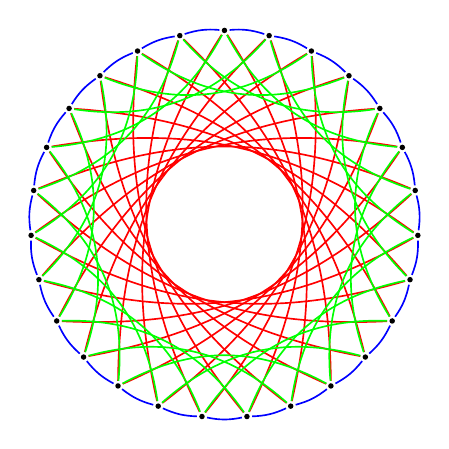
\begin{tikzpicture}[scale=.6,>=stealth,shorten >=.2mm,shorten <=.2mm,rotate=90,line width=.6pt]
          \isoggraph
        \end{tikzpicture}

        \vspace{.2ex}

        \only<3->{
          $\F_p$ \\[.7ex]
          \textbf{CSIDH}
          \,\raisebox{.2ex}{\small{[pron.: sea-side]}}
          \\ {\small
            \url{https://csidh.isogeny.org}
            \par}
        }
      \end{minipage}
      % 
      \begin{minipage}{.49\textwidth}\centering
        \begin{tikzpicture}[scale=2.456,>=stealth,shorten >=.2mm,shorten <=.2mm,rotate=90,line width=.6pt]
          \fpsqgraph
        \end{tikzpicture}

        \vspace{.2ex}

        \only<3->{
          $\F_{p^2}$ \\[.7ex]
          \textbf{SIDH}
          \\ {\small
            \url{https://sike.org}
            \par}
        }
      \end{minipage}

      \only<-2>{
        \vspace{3ex}

        \textit{Which of these is good for crypto?}
        \pause
        \onslide<2>{%
          \,\textbf{Both.}
        }
      }

    \end{center}
  \end{overlayarea}
\end{frame}
  
%%

\begin{frame}{CSIDH vs SIDH}
  \centering
  \vspace{-3mm}
  \begin{tabular}{l *{2}{| @{\hspace{1em}}c@{\hspace{1em}}} }
    & \textbf{CSIDH} & \textbf{SIDH}\\
    \hline
    Speed (on x64 arch., NIST 1) & $\sim$ 70ms & $\sim$ 6ms\\
    Public key size (NIST 1) & 64B & 346B\\
    Key compression & \\
    \enskip{}\rotatebox[origin=c]{180}{$\Lsh$} speed & & $\sim$ 11ms\\
    \enskip{}\rotatebox[origin=c]{180}{$\Lsh$} size & & 209B\\
    Submitted to NIST & no & yes\\
    TRL & 4 & 6\\
    \hline
    Best classical attack & $p^{1/4}$ & $p^{1/4}\;\;$ ($p^{3/8}$)\\
    Best quantum attack & $\tildO\left(3^{\sqrt{\log_3 p}}\right)$ & $p^{1/6}\;\;$ ($p^{3/8}$)\\
    Key size scales & quadratically & linearly\\
    CPA security & yes & yes\\
    CCA security & yes & Fujisaki-Okamoto\\
    Constant time & \alert<2->{it's complicated} & yes\\
    \hline
    Non-interactive key exchange & yes & no\\
    Signatures & short but (slow $\mid$ do not scale) & big and slow
  \end{tabular}
\end{frame}

%%

\begin{frame}{The CSIDH graph}
  \begin{center}
    \begin{tikzpicture}
      \begin{scope}
        \def\crater{12}
        \def\jumpa{-8}
        \def\jumpb{9}
        \def\diam{3cm}

        \foreach \i in {1,...,\crater} {
          \uncover<2->{\draw[blue] (360/\crater*\i : \diam) to[bend right] (360/\crater*\i+360/\crater : \diam);}
          \uncover<3->{\draw[red] (360/\crater*\i : \diam) to[bend right] (360/\crater*\i+\jumpa*360/\crater : \diam);}
          \uncover<4->{\draw[green] (360/\crater*\i : \diam) to[bend right=50] (360/\crater*\i+\jumpb*360/\crater : \diam);}
        }
        \foreach \i in {1,...,\crater} {
          \draw[fill] (360/\crater*\i: \diam) circle (2pt) +(360/\crater*\i: 0.4) node{$E_{\i}$};
        }
      \end{scope}
      \begin{scope}[xshift=5cm]
        \draw (0,2.5) node[anchor=west] {\parbox{6cm}{%
            Vertices are\\
            \emph{supersingular elliptic curves}\\
            over $\F_p$.\\[1em]
            \uncover<2->{Edges are \emph{isogenies}\\
              of bounded prime degree.}  }};
      
        \uncover<2->{\draw[blue] (0,0) -- (0.5,0)
          (0.5,0) node[anchor=west] {degree $3$};}
        \uncover<3->{\draw[red] (0,-1) -- (0.5,-1) (0.5,-1)
          node[anchor=west] {degree $5$};}
        \uncover<4->{\draw[green]
          (0,-2) -- (0.5,-2) (0.5,-2) node[anchor=west] {degree $7$};}
      \end{scope}
    \end{tikzpicture}
  \end{center}
\end{frame}

%%

\begin{frame}
  \frametitle{CSIDH key exchange}

  \begin{columns}
    \begin{column}{0.55\textwidth}
      \begin{tikzpicture}
        \begin{scope}
          \def\crater{12}
          \def\jumpa{-8}
          \def\jumpb{9}
          \def\diam{2.5cm}
          
          \foreach \i in {1,...,\crater} {
            \pgfmathparse{int(mod(2^\i,13))}
            \let\exp\pgfmathresult
            \draw[fill] (360/\crater*\i: \diam) circle (2pt);
          }
          \uncover<2,6->{
            % Alice 1
            \myedge{0}{1}{blue}\myedge{1}{5}{red}\myedge{5}{6}{blue}\myedge{6}{3}{green}
          }
          \uncover<3,5>{
            % Bob 1
            \begin{scope}[dashed,thick]
              \myedge{0}{4}{red}\myedge{4}{8}{red}\myedge{8}{5}{green}\myedge{5}{6}{blue}
            \end{scope}
          }
          \uncover<5>{
            % Alice 2
            \myedge{6}{7}{blue}\myedge{7}{11}{red}\myedge{11}{0}{blue}\myedge{0}{9}{green}
          }
          \uncover<6->{
            % Bob 2
            \begin{scope}[dashed,thick]
              \myedge{3}{7}{red}\myedge{7}{11}{red}\myedge{11}{8}{green}\myedge{8}{9}{blue}
            \end{scope}
          }

          \draw (0 : \diam + 0.4cm) node {$E_0$};
          \uncover<2->{\draw (360/\crater*3 : \diam + 0.4cm) node {$E_A$};}
          \uncover<3->{\draw (360/\crater*6 : \diam + 0.4cm) node {$E_B$};}
          \uncover<5->{\draw (360/\crater*9 : \diam + 0.4cm) node {$E_{BA}\uncover<6->{=E_{AB}}$};}
        \end{scope}
      \end{tikzpicture}  
    \end{column}    
    \begin{column}{0.45\textwidth}
      \textbf{Public parameters:}
      \begin{itemize}
      \item A supersingular curve $E_0/\F_p$;
      \item A set of small prime degree isogenies.
      \end{itemize}
      \begin{enumerate}
      \item<2-> \textbf{Alice} takes a \alert{secret} random walk
        \emph{$ϕ_A:E_0\to E_A$} of length \emph{$O(\log p)$};
      \item<3-> \textbf{Bob} does the same;
      \item<4-> They publish \emph{$E_A$} and \emph{$E_B$};
      \item<5-> \textbf{Alice} repeats her secret walk \emph{$ϕ_A$}
        starting from \emph{$E_B$}.
      \item<6-> \textbf{Bob} repeats his secret walk \emph{$ϕ_B$}
        starting from \emph{$E_A$}.
      \end{enumerate}
    \end{column}
  \end{columns}
\end{frame}

%%

\begin{frame}{CSIDH data flow}
  \textbf{Your secret:} a vector of number of \emph{isogeny steps} for each degree
  \begin{center}
    \begin{tikzpicture}
      \node at (0,0) {
        $\bigl( \bl{5}, \rd{1}, \gr{-4}, \dots \bigr)$
      };
      \begin{scope}[xshift=3cm,xscale=0.3,yscale=0.2]
        \draw (0,0) -- (18,0);
        \draw[dotted] (0,5) -- (18,5) (0,-5) -- (18,-5);

        \foreach \i in {0,...,18} {
          \pgfmathparse{round(5*sin(125*\i))}
          \let\r\pgfmathresult
          \draw[very thick] (\i,0) -- (\i,\r);
        }
      \end{scope}
    \end{tikzpicture}
  \end{center}
  
  \bigskip
  
  \textbf{Your public key:} (the $j$-invariant of) a supersingular elliptic curve
  \begin{align*}
    j =\;\; &\mathtt{0x23baf75419531a44f3b97cc9d8291a275047fcdae0c9a0c0ebb993964f821f2}\\
            &\mathtt{0c11058a4200ff38c4a85e208345300033b0d3119ff4a7c1be0acd62a622002a9}
  \end{align*}
\end{frame}

%%

\begin{frame}{Isogeny evaluation}
  \begin{columns}
    \begin{column}{0.45\textwidth}
      \textbf{Repeat:}
      \begin{itemize}
      \item Take a \emph{random point} $P\in E(\F_p)$;
      \item Set \emph{$Q=[c]P$},\\
        where \emph{$c$} is an \emph{appropriate cofactor}, so that
        \emph{$N = \#〈Q〉$} contains only \emph{useful} prime
        factors;
      \item Advance by the \emph{degree $N$} isogeny of \emph{kernel
        $〈Q〉$}.
      \end{itemize}
    \end{column}  
    \begin{column}{0.4\textwidth}
      \centering
      \transdissolve<2->
      \begin{tikzpicture}
        \begin{scope}
          \def\crater{12}
          \def\jumpa{-8}
          \def\jumpb{9}
          \def\diam{2cm}
          
          \foreach \i in {1,...,\crater} {
            \pgfmathparse{int(mod(2^\i,13))}
            \let\exp\pgfmathresult
            \draw[fill] (360/\crater*\i: \diam) circle (2pt);
          }

          \draw (0 : \diam + 0.4cm) node {$E_0$};
          \uncover<18>{\draw (360/\crater*8 : \diam + 0.4cm) node {$E_A$};}
          
          \uncover<3-5,18>{
            \myedge{0}{1}{blue}\myedge{1}{5}{red}
            \myedge{5}{2}{green}\myedge{2}{9}{orange}
          }
          \uncover<6-8,18>{
            \myedge{9}{10}{blue}\myedge{10}{2}{red}\myedge{2}{11}{green}
          }
          \uncover<9-11,18>{\myedge{11}{8}{green}}
          \uncover<12-14,18>{\myedge{8}{0}{red}}
          \uncover<15-16,18>{\myedge{0}{4}{red}}
          \uncover<17->{\myedge{4}{8}{red}}
        \end{scope}

        \begin{scope}[yshift=-3cm]
          \uncover<2-3>{
            \node at (0,0) {$\#〈P〉 = \bl{3}\cdot\rd{5}\cdot\gr{7}\cdot\og{11}$};
          }
          \uncover<3>{
            \node at (0,-1) {$Q = P$}; 
          }
          \uncover<5-6>{
            \node at (0,0) {$\#〈P〉 = \bl{3}\cdot\rd{5}\cdot\gr{7}\cdot\og{11}$};
            \node at (0,-1) {$Q = [\og{11}]P$};
          }
          \uncover<8-9>{
            \node at (0,0) {$\#〈P〉 = \bl{3}\cdot\gr{7}\cdot\og{11}$};
            \node at (0,-1) {$Q = [\bl{3}\cdot\og{11}]P$};
          }
          \uncover<11,12,14,16>{
            \node at (0,0) {$\#〈P〉 = \bl{3}\cdot\rd{5}\cdot\gr{7}\cdot\og{11}$};
            \node at (0,-1) {$Q = [\bl{3}\cdot\gr{7}\cdot\og{11}]P$};
          }
        \end{scope}
        
        \begin{scope}[xshift=2.5cm,yshift=-3.5cm,xscale=0.3,yscale=0.2]
          \draw (0,0) -- (4,0);
          \draw[dotted] (0,5) -- (4,5) (0,-5) -- (4,-5);

          \uncover<-3,18>{\sk{2}{5}{-3}{1}}
          \uncover<4-6>{\sk{1}{4}{-2}{0}}
          \uncover<7-9>{\sk{0}{3}{-1}{0}}
          \uncover<10-12>{\sk{0}{3}{0}{0}}
          \uncover<13-14>{\sk{0}{2}{0}{0}}
          \uncover<15-16>{\sk{0}{1}{0}{0}}
        \end{scope}
      \end{tikzpicture}
    \end{column}
  \end{columns}
\end{frame}

%%

\begin{frame}{In seek of constant time}
  \textbf{Two obstacles for constant time:}
  \begin{enumerate}
  \item \alt<2->{\sout{Some random points $P$ may lack some factors;}
      \hfill\emph{Unrelated to secret key if truly random.}} {Some random points $P$ may lack
      some factors;}
  \item Number of isogeny evaluations dependent on secret key.
  \end{enumerate}
  
  \begin{block}{Meyer, Campos, Reith 2018; Onuki, Aikawa, Yamazaki, Takagi 2019}<3->
    \begin{itemize}
    \item \emph{``Dummy'' isogenies:}
      \begin{itemize}
      \item Always do exactly the same number of isogeny evaluations per prime degree,
      \item discard computations in excess;
      \end{itemize}
    \item \emph{$4×$} slowdown (MCR) / \emph{$2.5×$} slowdown (OAYT).
    \item Protected against SPA\dots \uncover<4->{but \emph{very easy to attack by fault!}}
    \end{itemize}
  \end{block}
\end{frame}

%%

{
  \setbeamercolor{background canvas}{bg=black}
  \begin{frame}[plain]
    \begin{tikzpicture}[remember picture,overlay]
      \node(pic)[at=(current page.center)] {
        \includegraphics[width=\paperwidth]{dummy.jpg}
      };
    \end{tikzpicture}
  \end{frame}
}

%%

\begin{frame}{Isogeny evaluation with dummies}
  \centering
  \transdissolve<2->
  \begin{tikzpicture}
    \begin{scope}
      \def\crater{12}
      \def\jumpa{-8}
      \def\jumpb{9}
      \def\diam{3cm}
      
      \foreach \i in {1,...,\crater} {
        \pgfmathparse{int(mod(2^\i,13))}
        \let\exp\pgfmathresult
        \draw[fill] (360/\crater*\i: \diam) circle (2pt);
      }

      \draw (0 : \diam + 0.4cm) node {$E_0$};
      \uncover<8>{\draw (360/\crater*8 : \diam + 0.4cm) node {$E_A$};}
      
      \uncover<2,8>{
        \myedge{0}{1}{blue}\myedge{1}{5}{red}
        \myedge{5}{2}{green}\myedge{2}{9}{orange}
      }
      \uncover<3,8>{
        \myedge{9}{10}{blue}\myedge{10}{2}{red}\myedge{2}{11}{green}
        \myedge{11}{6}{orange,dashed}
      }
      \uncover<4,8>{
        \myedge{11}{8}{green}
        \myedge{8}{9}{blue,dashed}\myedge{9}{1}{red,dashed}\myedge{1}{8}{orange,dashed}
      }
      \uncover<5,8>{
        \myedge{8}{0}{red}
        \myedge{0}{1}{blue,dashed}\myedge{1}{10}{green,dashed}\myedge{10}{5}{orange,dashed}
      }
      \uncover<6,8>{
        \myedge{0}{4}{red}
        \myedge{4}{5}{blue,dashed}\myedge{5}{2}{green,dashed}\myedge{2}{9}{orange,dashed}
      }
      \uncover<7->{
        \myedge{4}{8}{red}
        \myedge{8}{9}{blue,dashed}\myedge{9}{6}{green,dashed}\myedge{6}{1}{orange,dashed}
      }
    \end{scope}

    \begin{scope}[xshift=7cm,yshift=1.5cm]
      \uncover<2-3,5->{
        \node at (0,0) {$\#〈P〉 = \bl{3}\cdot\rd{5}\cdot\gr{7}\cdot\og{11}$};
      }
      \uncover<4>{
        \node at (0,0) {$\#〈P〉 = \bl{3}\cdot\gr{7}\cdot\og{11}$};
      }
    \end{scope}
    
    \begin{scope}[xshift=7cm,yshift=-1.5cm,xscale=0.3,yscale=0.2]
      \draw (0,0) -- (4,0);
      \draw[dotted] (0,5) -- (4,5) (0,-5) -- (4,-5);

      \uncover<1-2,8>{\sk{2}{5}{-3}{1}}
      \uncover<3>{\sk{1}{4}{-2}{0}}
      \uncover<4>{\sk{0}{3}{-1}{0}}
      \uncover<5>{\sk{0}{3}{0}{0}}
      \uncover<6>{\sk{0}{2}{0}{0}}
      \uncover<7>{\sk{0}{1}{0}{0}}
    \end{scope}
  \end{tikzpicture}
\end{frame}

%%

\begin{frame}{Our work (Latincrypt 2019)}
  \begin{itemize}
  \item<+-> \emph{Fixed a leak} related to the sampling of random points.
  \item<+-> \emph{Speed-up} both MCR and OAYT constant time implementations:
    \begin{itemize}
    \item Fully \emph{Twisted Edwards} implementation;
    \item Use of \emph{Shortest Differential Addition Chains};
    \end{itemize}
  \item<+-> \emph{Protection} against \emph{fault} attack at the cost of a
    $2×$ slowdown:
    \begin{itemize}
    \item Got rid of ``dummy isogenies''.
    \end{itemize}
  \item<+-> Initiated study of \emph{fully constant time} variant
    (very expensive, though).
  \end{itemize}
\end{frame}

%%

\begin{frame}{Avoiding dummies}
  We change the format of the secret key:
  \begin{description}
  \item[Original:] vectors with coefficients in $[-B,B]$.
  \item[Modified:] vectors with \emph{odd}\footnote{Or \emph{even},
      all the same.} coefficients in $[-B,B]$.
    \begin{itemize}
    \item<2-> Translate vector to \emph{sum of $±1$ vectors};
    \item<2-> Each vector costs exactly \emph{one isogeny evaluation} per
      degree.
    \end{itemize}
  \end{description}

  \bigskip
  
  \begin{center}
    \begin{tikzpicture}[xscale=0.4,yscale=0.3]
      \begin{scope}
        \draw (0,0) -- (3,0);
        \draw[dotted] (0,5) -- (3,5) (0,-5) -- (3,-5);
        \sk{3}{5}{-3}{1}
        \node at (0,6) {\footnotesize$\bl{3}$};
        \node at (1,6) {\footnotesize$\rd{5}$};
        \node at (2,6) {\footnotesize$\gr{-3}$};
        \node at (3,6) {\footnotesize$\og{1}$};
      \end{scope}

      \bigskip
      \begin{uncoverenv}<2->
        \node at (6,0) {\Large $=$};

        \begin{scope}[xshift=8cm]
          \draw (0,0) -- (3,0);
          \sk{1}{1}{-1}{1}
        \end{scope}

        \node at (13,0) {\Large $+$};
        \begin{scope}[xshift=14cm]
          \draw (0,0) -- (3,0);
          \sk{1}{1}{-1}{1}
        \end{scope}

        \node at (19,0) {\Large $+$};
        \begin{scope}[xshift=20cm]
          \draw (0,0) -- (3,0);
          \sk{1}{1}{-1}{-1}
        \end{scope}

        \node at (25,0) {\Large $+$};
        \begin{scope}[xshift=26cm]
          \draw (0,0) -- (3,0);
          \sk{1}{1}{-1}{1}
        \end{scope}

        \node at (31,0) {\Large $+$};
        \begin{scope}[xshift=32cm]
          \draw (0,0) -- (3,0);
          \sk{-1}{1}{1}{-1}
        \end{scope}
      \end{uncoverenv}
    \end{tikzpicture}
  \end{center}
\end{frame}

%%

\begin{frame}{Summary}
  \Large
  \begin{itemize}
    \setlength{\itemsep}{1em}
  \item Repeat with me: \emph{I need isogeny-based crypto!}
  \item \emph{CSIDH} is the new Diffie--Hellman:\\
    Very short keys, easy key validation, \dots
  \item Implementing isogeny-based crypto \emph{efficiently} is
    challenging,\\
    even more so with \emph{side-channel protections}.
  \end{itemize}
\end{frame}

%%

\begin{frame}[plain]
  \centering
  \begin{tikzpicture}[remember picture,overlay]
    \begin{scope}[xscale=1.7,yshift=-15,opacity=0.8]
      \def\crater{12}
      \def\jumpa{-8}
      \def\jumpb{9}
      \def\diam{5cm}

      \foreach \i in {1,...,\crater} {
        \draw[blue] (360/\crater*\i : \diam) to[bend right] (360/\crater*\i+360/\crater : \diam);
        \draw[red] (360/\crater*\i : \diam) to[bend right] (360/\crater*\i+\jumpa*360/\crater : \diam);
        \draw[green] (360/\crater*\i : \diam) to[bend right=50] (360/\crater*\i+\jumpb*360/\crater : \diam);
      }
    \end{scope}
    
    \draw (0,0.5) node{\Huge\bf Thank you};
    \draw (0,-1.1) node{\large\url{https://defeo.lu/}};
    \draw (0,-1.8) node{\large\includegraphics[height=0.9em]{twitter.png}~\href{https://twitter.com/luca_defeo}{@luca\_defeo}};
  \end{tikzpicture}
\end{frame}

\end{document}


% LocalWords:  Isogeny abelian isogenies hyperelliptic supersingular Frobenius
% LocalWords:  isogenous


